% For ODBASE Submission:
% Paper id: 20
% Password: a37ebf

%%%%%%%%%%%%%%%%%%%%%%% file typeinst.tex %%%%%%%%%%%%%%%%%%%%%%%%%
%
% This is the LaTeX source for the instructions to authors using
% the LaTeX document class 'llncs.cls' for contributions to
% the Lecture Notes in Computer Sciences series.
% http://www.springer.com/lncs       Springer Heidelberg 2006/05/04
%
% It may be used as a template for your own input - copy it
% to a new file with a new name and use it as the basis
% for your article.
%
% NB: the document class 'llncs' has its own and detailed documentation, see
% ftp://ftp.springer.de/data/pubftp/pub/tex/latex/llncs/latex2e/llncsdoc.pdf
%
%%%%%%%%%%%%%%%%%%%%%%%%%%%%%%%%%%%%%%%%%%%%%%%%%%%%%%%%%%%%%%%%%%%

\documentclass[runningheads,a4paper,11pt]{llncs}

\usepackage{amssymb}
\usepackage{graphicx}
\usepackage{paralist}
\usepackage{amsmath}
\usepackage{array}
\usepackage[hidelinks]{hyperref}

\usepackage{listings}
\usepackage{booktabs}
\usepackage[labelfont=bf]{caption}

% % % non-llncs modules % % %

\usepackage{longtable}
\usepackage{tabularx}
\usepackage{everysel}
\usepackage{xtab}
\usepackage{ragged2e}
\usepackage{everysel}
\usepackage{url}
\usepackage{datetime}
\usepackage{setspace}
\usepackage{rotating}

% define some fancy checkmarks
\usepackage{pifont}% http://ctan.org/pkg/pifont
\newcommand{\cmark}{\ding{52}}%
\newcommand{\xmark}{\ding{56}}%

% customize margins
\usepackage{anysize}
\marginsize{1in}{1in}{1in}{1in}

% customize line spacing
\usepackage{setspace}
\onehalfspacing

% % % % % % % % % % % % % % % 


\makeatletter
\newcommand{\thickhline}{%
    \noalign {\ifnum 0=`}\fi \hrule height 1pt
    \futurelet \reserved@a \@xhline
}
\makeatother

\usepackage{url}
\urldef{\mailsa}\path|martini@cs.uoregon.edu|
\urldef{\mailsb}\path|author2@someotherinst.something|
\urldef{\mailsc}\path|author3@someotherinst.something|
\newcommand{\keywords}[1]{\par\addvspace\baselineskip
\noindent\keywordname\enspace\ignorespaces#1}

\begin{document}

\mainmatter  % start of an individual contribution

% first the title is needed
\title{Predicting Atom Positions Using \\\vspace{.5em} Machine Learning Algorithms}


% the name(s) of the author(s) follow(s) next
%
% NB: Chinese authors should write their first names(s) in front of
% their surnames. This ensures that the names appear correctly in
% the running heads and the author index.
%
\author{Adam Martini, Wes Erickson, Ran Tian}
\institute{Computer and Information Science Department\\
University of Oregon\\ Eugene, Oregon 97403, USA \\ \mailsa \\ \mailsb \\ \mailsc}


%
% NB: a more complex sample for affiliations and the mapping to the
% corresponding authors can be found in the file "llncs.dem"
% (search for the string "\mainmatter" where a contribution starts).
% "llncs.dem" accompanies the document class "llncs.cls".
%

\maketitle

\begin{abstract} Here is an abstract...
\keywords{machine learning, logistic regression, ...}
\end{abstract}

\section{Introduction}

The Steck Lab is investigating the motion of a single atom in a Magneto Optical Trap (MOT).  The atom is imaged using a pair of aspheric lenses and a CCD camera.  Given an 2D image from the CCD, the lab wants to predict the probability distribution of the atom's location within the MOT. The lab consists of several individual parts including preprocessing, ray tracer generator and classifier. The subgoal of this lab is to distribute and integrate the individual parts.

This report describes our efforts to both simulate atom images, and to create a scalable probabilistic classifier capable of atom location prediction.  Section \ref{design} provides an overview of our system design and objectives.  We discuss the details of our development and implementation efforts in Section \ref{development}.  Experimental results are outlined in Section \ref{experiments} followed by an discussion of the lessons learned in Section \ref{lessons}. We conclude the report in Section \ref{conclusion}.

\section{Design and Objectives}
\label{design}

To tackle this problem we run simulations of the CCD output for a given atom location using a raytracing simulation.  The output images are labeled according to atom location and used as training data for machine learning algorithms to create classification models.  The models can then be used to generate a probabilistic distribution for the atom's location for a new CCD image.  

Figure \ref{fig:arch} describes the data flow of our architecture.  We begin by simulating the training and testing data using raytracing and filtering.  The filters will apply both generate several different training sets from a single image set.  The classification results for each training set are described below.  Some of the instances are selected from the image set for noise filtering.  The \emph{noisy} data is used to test our classification algorithms.

\begin{figure}[h]
\begin{center}
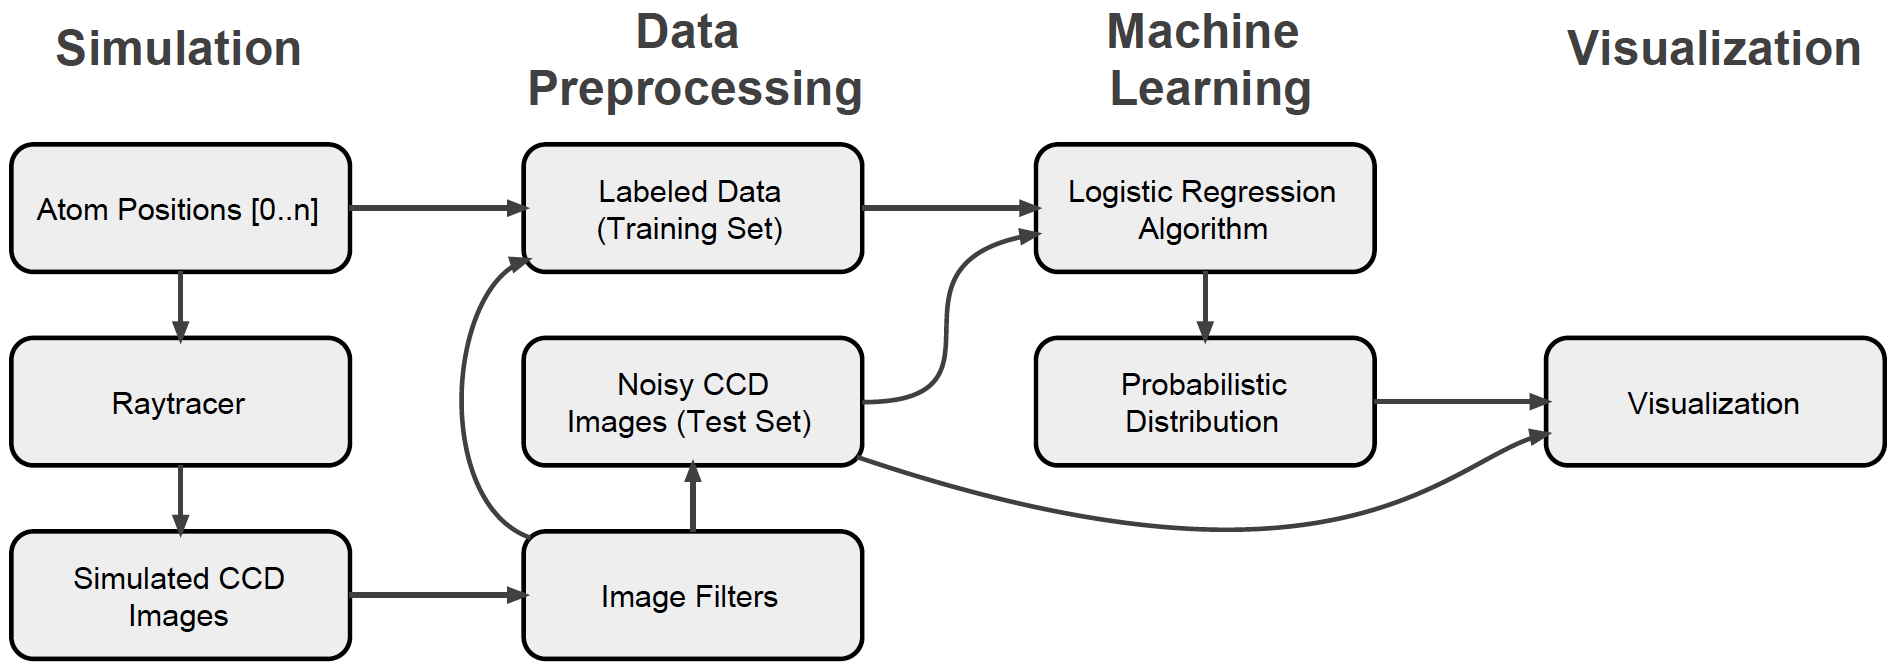
\includegraphics[scale=0.4]{arch.png}
\caption{High Level Data Flow Architecture Diagram}
\label{fig:arch}
\end{center}
\end{figure}

The objective of our project is to create and test a scalable machine learning solution for atom location prediction using CCD images.  In order to scale our application we use both shared memory and distributed memory parallelism.  Massive amounts of training data are generated using a shared memory parallelism, and a distributed memory logistic regression classifier is used to efficiently learn interesting patterns from the data.  The remainder of this report describes our development efforts, experimentation results, and the lessons we have learned during the process.

\section{Development and Implementation}
\label{development}

Our development efforts are divided into sections based on our data flow architecture.  There is some overlap of effort in the data preprocessing step as this is the area of our development where Simulation and Machine Learning meet.  We describe each development stage in detail in the following subsections.

\subsection{Simulation}

Wes talks about simulations here ...

OLD TEXT:
The essence of the simulation is starting with a flourescent atom at a chosen location, and then simulating how light emitted from the atom appears on the CCD. There are two approaches to simulating the generation of CCD images from a given atom location.

The first is a classical raytracing approach. Rays are emitted in a random direction from the atom, and obey refraction via Snell's Law as they pass interfaces between different materials. The rays also contain phase information for the purposes of determining interference. When the rays intersect with the CCD plane, we increment an array value corresponding to which CCD pixel it hit.

The second approach is a full simulation of the linear wave equation. This is a full 3D simulation, and is much more computationally intensive. A field discretized into $~200\times 200\times 1000$ is given an initial value of zero everywhere except for a peak at our atom location, and then is stepped forward in time according to the linear wave equation. The essence of this algorithm is basic matrix multiplication, but with very large sparse matrices.

\subsection{Data Preprocessing}

%Ran talks about filtering here...
The original picture is designed to be 100 times 100 pixels matrix in each slice. The data preprocessing build a noise maker and filtering mechanism before the slices of matrix are actually applied to the classifier. It actually simulates a half transparent mask before the camera practically. The image generated by such mask adds Poisson distributed random number to every pixels of the image. A Poisson distribution stands for discrete probability that can give a number of events occurring in a fixed interval of time or space if events are independent with the average of $\lambda$. The value of $\lambda$ is switched between different proposed number in real test. Filtering, on the other hand, is clearing the influence caused by the noises. The filtering mechanism generally follows the work in course lab 8. A Gaussian distribution based figure blur decreases the degree of distribution caused by Poisson distribution based noises. Then, the Prewitt gradient filters all unnecessary noise with only structure, which contains the lines of rays, left.

The feature scaling step is handled in the logistic regression classifier as it is a simple extension to data loading after the instance have been loaded into memory.  We use efficient a C++ template library for linear algebra \cite{Eigen} that provides efficient matrix operations that can quickly perform the broadcasting operations necessary for feature scaling.  In addition, the distributed implementation of our algorithm lends itself well to efficient data partitioning, which ensures that this preprocessing step will scale.  However, feature scaling in a distributed setting is slightly more complex in that it requires knowledge of the global min and max for the entire dataset across all nodes.  The min/max vectors is quickly computed using an Allreduce step with MPI's MIN/MAX reduction operators. Each node then formats its section of the data using a single call feature scaling utility function.

\subsection{Machine Learning}
We have developed a distributed logistic regression classifier using MPI to train on massive amounts of data efficient.  The classifier is capable of multi-class classification and mini-batch processing.  During training, nodes communicate with each other to both build the model and perform parameter updates.

The model building step includes data loading, feature scaling, and label formating. During data loading, each node loads a portion of the instances the provided data directory based on its task ID and the total number of tasks in the communication world.  It is important to note that the instance file names are first loaded into a vector and then randomized to ensure that mini-batch processing have a consistent sample of the data with each iteration.  After the data is loaded, feature scaling is performed as described above.  The label formating step uses a custom MPI operator in an Allreduce call to generate global unique label set.  The unique label set is used at each node to generate a label matrix from the label vector for 1-vs-all classification.

The model training involves iterative updates to a set of global parameters.  During each update, the nodes compute a portion gradient update using a subset of the data they are responsible for based on the batch size.  The collective gradient update is computed using an Allreduce call to sum each contribution followed by a normalization step on each node based on the total number of instances contributing to the update.  The new parameter set (identical on all nodes) is then tested for convergence and used for the next iteration.

Training is finished when either the gradient has converged or the maximum number of iterations has been reached.  The Master node saves the trained model parameters to the a file to be loaded on a single node for testing.  The testing program generates a set of class membership probabilities for each instance in the given data directory.  The chosen class is simply the maximum probability found in the probabilities set for each instance.  We also use the probabilities to generate the visualizations of the models \emph{beliefs} about an atoms location for each instance.

\subsection{Visualization}
Visualization is particularly important for visualizing three dimensional volumes, and it may become essential for feedback as to whether our simulations are functioning properly, and for our presenting our project results. However, our project focus is not on programming the visualization methods ourselves, but using existing tools such as Visit or ParaView.

The main items to be visualized are the field generated from the differential equation solvers, and the CCD images (which are a cross section of the field). We can also use these tools for post processing on the image data to highlight features for the benefit of the machine learning algorithm.

\section{Experiments and Performance}
\label{experiments}

\subsection{Raytracing}

Initial tests of the raytracer.

\begin{figure}
\centering
\begin{subfigure}{.5\textwidth}
  \centering
  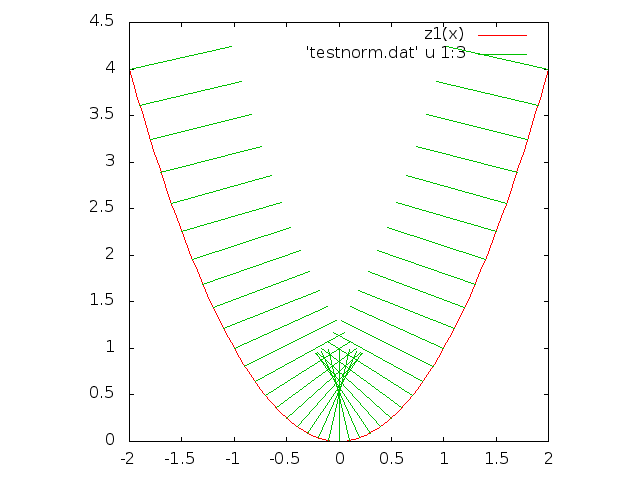
\includegraphics[width=7cm]{out.png}
  \caption{A norm}
  \label{fig:sub1}
\end{subfigure}%
\begin{subfigure}{.5\textwidth}
  \centering
  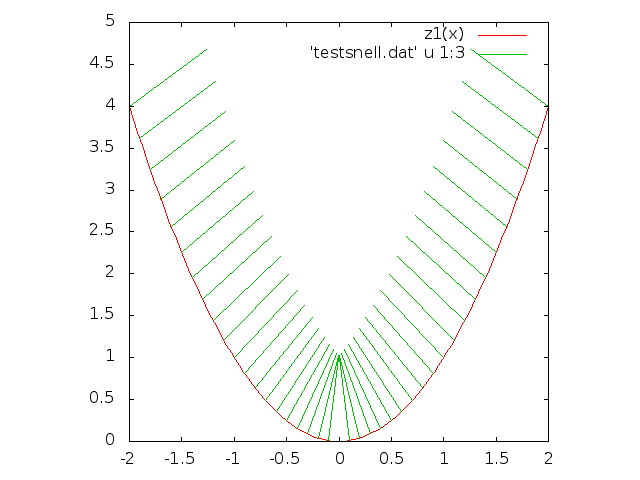
\includegraphics[width=7cm]{out2.png}
  \caption{A snell}
  \label{fig:sub2}
\end{subfigure}
\caption{A figure with two subfigures}
\label{fig:test}
\end{figure}

\begin{figure}
\centering
\begin{subfigure}{.5\textwidth}
  \centering
  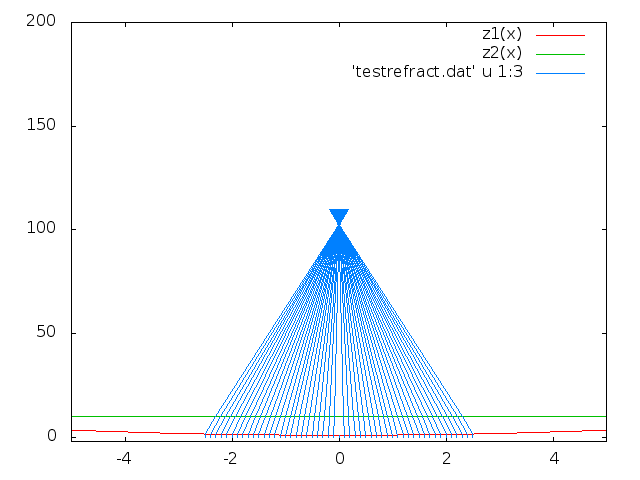
\includegraphics[width=7cm]{out4.png}
  \caption{A refract}
  \label{fig:sub3}
\end{subfigure}%
\begin{subfigure}{.5\textwidth}
  \centering
  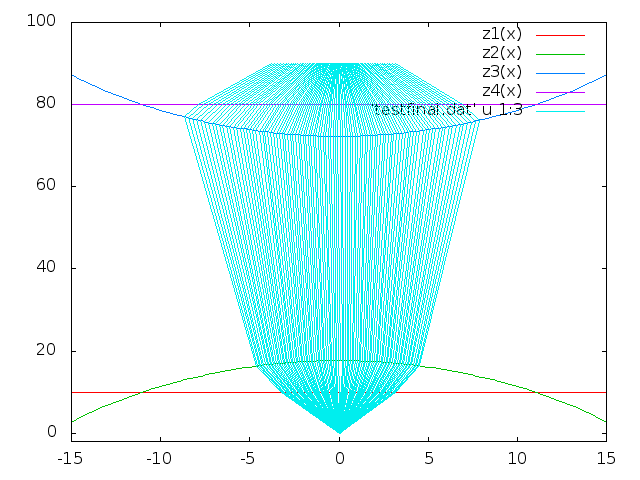
\includegraphics[width=7cm]{out5.png}
  \caption{A lenstest}
  \label{fig:sub4}
\end{subfigure}
\caption{A figure with two subfigures}
\label{fig:test2}
\end{figure}



\subsection{Training and Regression}

We had limited time to perform experiments due to the late arrival of our dataset.  However, the tests that we did perform clearly show that our distributed logistic classifier scales well to achieve significant performance gains.  In addition to provable performance gains, we also observed Gustafson's Law in action in that the available parallelism significantly increases with our problem size.

For our initial tests, we ran two training sets through the classifier.  The first training set was small (283M) and the second set was larger (~2.9G).  Our first goal was to observe the classification accuracy on of the classifier on the testing set.  Using the small training set, we were easily able to achieve 100\% accuracy.  This indicates that the amount of noise was insufficient and/or that there were not enough rays sampled to adequately obscure label partition boundaries.

Figures \ref{fig:small} \ref{fig:big} show performance gains for our initial tests.  We clearly see that while available parallelism levels out around 10 nodes with a student account on ACISS, the amount of available parallelism dramatically increases with our problem size.  The small dataset achieves a speedup of ~7 times relative to the serial execution while the larger dataset achieves ~9 times speed up.  This is an embarrassingly parallel problem with limited communication demands, so it is reassuring to see almost 10 times speedup with 10 times the computational power.  This implies that our implementation efficiently utilizes the parallel processing power to take advantage of available parallelism.

\begin{figure}[h]
\begin{center}
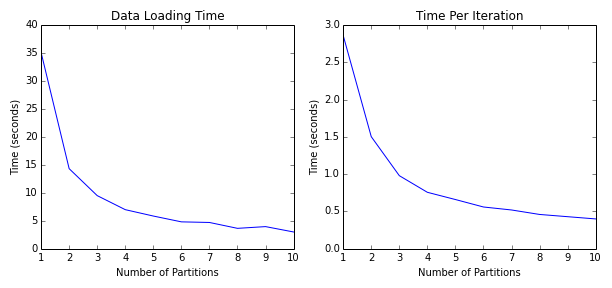
\includegraphics[scale=0.7]{small_metrics.png}
\caption{Performance gains for both data loading and iteration time on the small training set.}
\label{fig:small}
\end{center}
\end{figure}

\begin{figure}[h]
\begin{center}
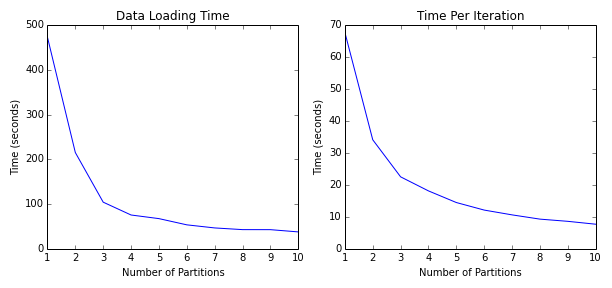
\includegraphics[scale=0.7]{big_metrics.png}
\caption{Performance gains for both data loading and iteration time on the large training set.}
\label{fig:big}
\end{center}
\end{figure}

\subsection{Visualization}

\begin{figure}
  \centering
  \includegraphics[scale=0.7]{ccd2D.png}
\end{figure}

\begin{figure}
\centering
\begin{subfigure}{.5\textwidth}
  \centering
  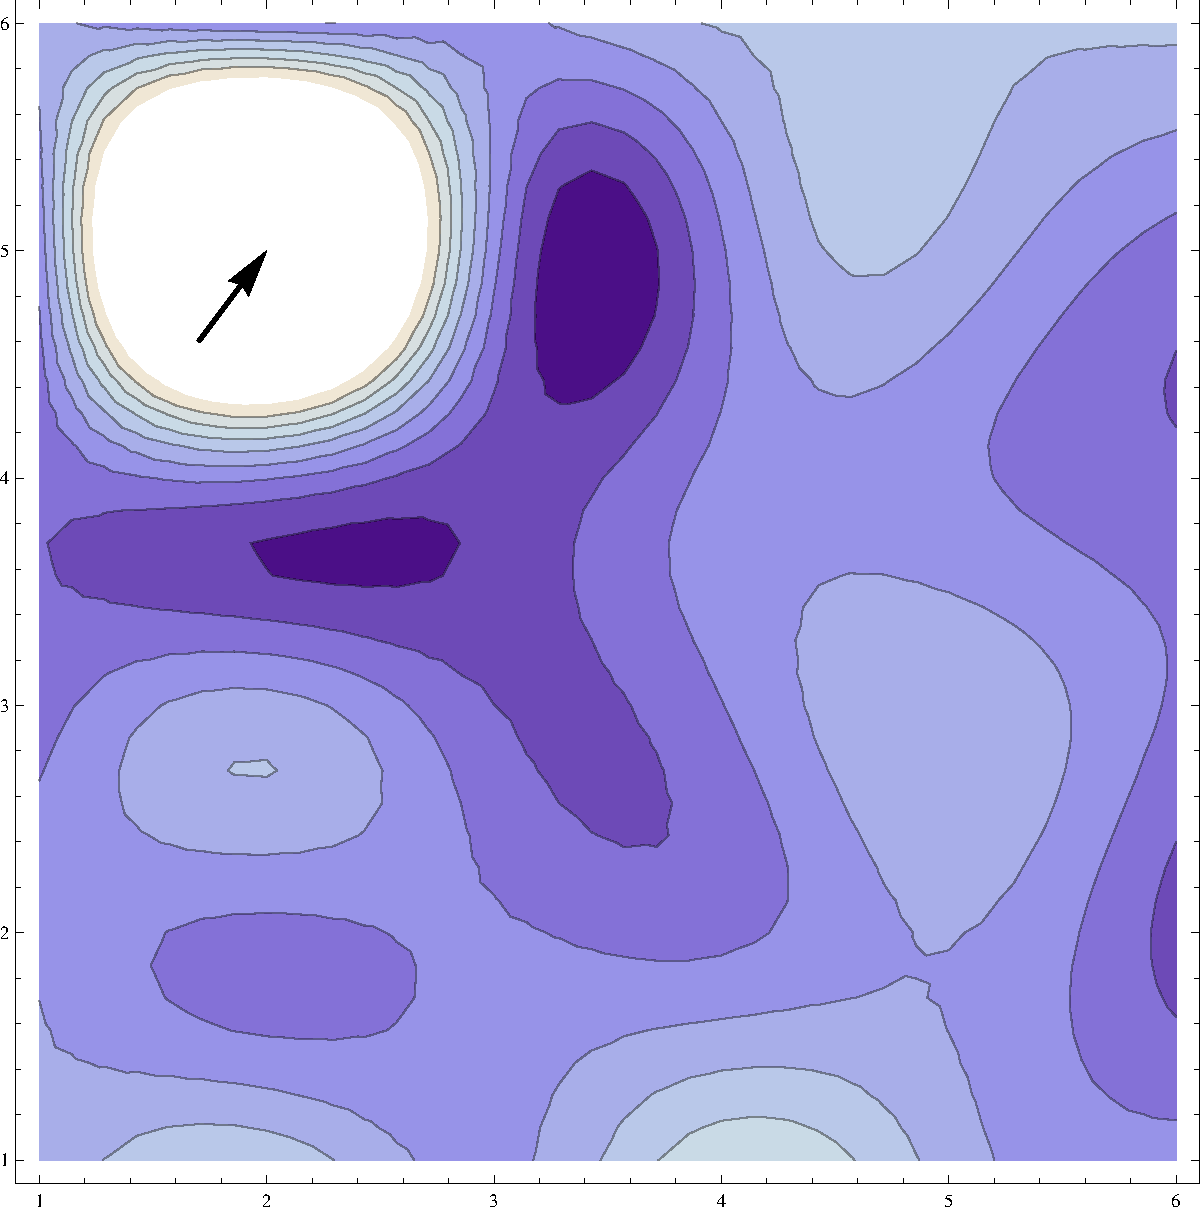
\includegraphics[scale=.35]{2-5.pdf}
\end{subfigure}%
\begin{subfigure}{.5\textwidth}
  \centering
  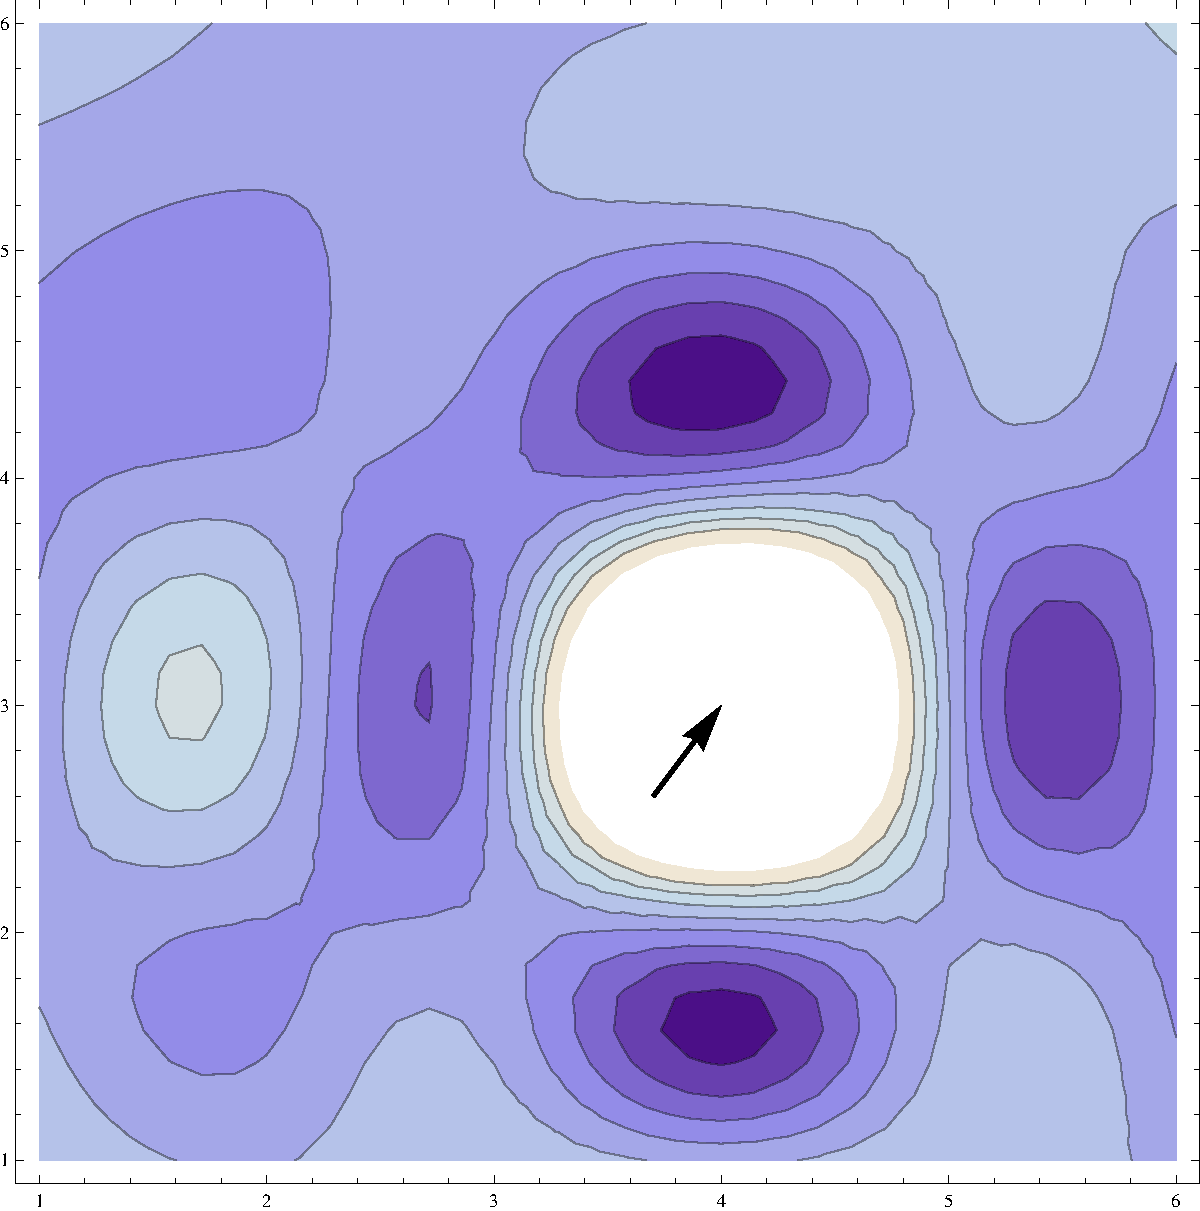
\includegraphics[scale=.35]{4-3.pdf}
\end{subfigure}
\label{fig:test2}
\end{figure}


\section{Lessons Learned}
\label{lessons}

\subsection{Simulation}


\subsection{Data Preprocessing}

%Ran talks about filtering here...
Sharing the idea and details of the implementation of Poisson distribution based noise maker is quite a job. Due to lack of base support of Poisson distribution random number generator, a float number and the range of the floating number is quite interesting topic. The final result turns out to be a integer generator with a scaling shifting. Hence, we can satisfy our purpose and simplify the implementation at same time.

%Adam talks about feature scaling here...
To accomplish distributed feature scaling and label formating we need to need to create a custom MPI reduce operation that is capable of merging two sets of labels into a single unique set.  We learned that creating custom reducers can be the source of many bugs related to incorrect data pointers.  This was also the case when created custom reducers for gradient updates, which we discuss below.

\subsection{Machine Learning}

%Ran talks about filtering here...
The origin plan includes another distributed memory system based classifier, which is distributed Support Vector Machine (SVM). The distributed SVM is a backup as a classifier for training and testing the ray images. However, after three weeks of work, the result turns out to be unacceptable. The implementation of distributed SVM contains a large number of interfaces that allows user to train and test the result. The only function our project needs is a regression mode for the 100 times 100 pixels image classifier. However, the regression mode does not support such simple functions after parsing the SVM Light files. The implementation complexes this part into more detailed partial differential equation classifier. Therefore, the decision between continuing the work to implement a corresponding function and stop to switch focusing on other object becomes quite controversial. Due to time limit and tight schedule of my last three weeks. Lacking of machine learning knowledge, I spend too much time studying on basic concept of SVM. The lesson I learnt is to better schedule the timeline and estimate the workload for a totally new area.



\subsection{Visualization}


\section{Conclusions}
\label{conclusion}
This report covers our work on a distributed logistic regression classifier to predict atom locations given CCD images.  We implemented a parallelized raytracer to simulate a large number of images that we then preprocessed to create out training and testing.  Successfully implemented and tested our distributed logistic regression classifier using the training and testing data to achieve 100\% accuracy.  Finally, we produced several visualizations to demonstrate classifier efficacy and parallel performance.


%------------------------------------------------------------------------

\bibliographystyle{plain}
\bibliography{references}

\end{document}